\documentclass[a4paper,12pt]{article}
\usepackage{biblatex}
\usepackage{listings}
\usepackage{graphicx}
\graphicspath{ {./} }
\title{Assignment 2 - Databases}
\date{2021\\April}
\author{Frederik Lassen}


\begin{document}
\maketitle
\thispagestyle{empty}
\clearpage
\pagenumbering{arabic}

\tableofcontents
\clearpage

\section{(Q)Task 1 - Investigation}
Produce a small writeup (around 300 words) answering the following questions. \\
\begin{enumerate}
\item What is point of NoSQL databases?
\item What is the CAP theorem?
\item What are ideal use cases of HBase?
\end{enumerate}

\section{(A)Task 1 - Investigation}
NoSQL databases was created because programmers weren’t content with SQL. NoSQL is easier scalable, easy datamodelling and the highest of uptimes. NoSQL stores its data in JSON formatted documents, and doesn’t use the conventional columns and rows that SQL uses. But of course NoSQL isn’t totally perfect, everything has its flaws. If you want the reliability of a relational database in your NoSQL database, it could be a very complex procedure. NoSQL is also not compatible with SQL, and also generally NoSQl is newer and as such, haven’t been as developed to the same extent relational databases have. This leads us to the CAP theorem which is an idea from a computer scientist, Eric Brewer, that explains that in computer systems you can’t satisfy all guarantees, those being availability, consistency and partition tolerance. This is explained in an example by the “two out of three” rule, whereas you want availability, consistency and partition tolerance but you can only have 2 of the 3 guarantees. 
Hbase is a NoSQL database that can store large qualities of sparse data, which is basically a very small amount of information kept in a very large set of not important data. Hbase is best used as a database where very large amounts of data is added consistently and needs to be handled without the database deteriorating. Some examples could be; Hbase is used actively for CDP by many companies and by banking institutions for checking for fraud in transactions. It is also used for long term storage, as well as hen data is generally too large to comfortably scale using traditional technologies.


\clearpage

\section{(Q)Task 2 - Bloom filters}
Bloom filters are used in hbase as an incredible optimization. Solve the following. \\
\begin{enumerate}
\item What is a bloom filter?
\item What is an advantage of bloom filters over hash tables?
\item What is a disadvantage of bloom filters?
\item Using your language of choice, implement a bloom filter with add and
check functions. The backing bit-array can simply be a long (64 bit
integer).
\item If you are to store one million ASCII strings with an average size of 10
characters in a hash set, what would be the approximate space consumption?
\item The following equation gives the required number of bits of space per
inserted key, where E is the false positive rate.
b = 1.44log2(1/E) (1)
\item How many bits per element are required for a 1\% false positive rate?
\item How many bits per element are required for a 5\% false positive rate?
\item If you are to store one million ASCII strings with an average size of 10
characters in a bloom filter, what would be the approximate space consumption, given an allowed false positive rate of 5\% ?.
\end{enumerate}

\section{(A)Task 2 - Bloom filters}
\begin{enumerate}
\item A Bloom filters checks whether an element is a member of a specific set. So it will either return a possible in set or a definitely not in set. It is probabilistic in nature.
\item Bloom filters dont store elements themselves. You dont test whether something is present, but rather if it is certainly not present. Bloom filters are mroe space-efficient than hash-tables: bloom filter uses many hash functions.
\item false negative potential. It can only say yes/no. No memory.
\item implement a bloom filter NOT DONE!
\item Assuming 1 string would be 56 bytes, the space consumption would be 56 000 000 bytes. which is roughly 53MB. 
\item Not a question
\item Fewer than 10 bits per element is required for a 1\% false positive probability(not rate).
\item Using a calculator assuming 1000000 elements it would be around 19 bits per element for a 5\%  probability for a false positive(1 hash function)
\item 1MB (har brugt denne til 3 af opgaverne: https://hur.st/bloomfilter/)
\end{enumerate}

\clearpage

\section{(Q)Task 3 - Huffman coding}

HBase internally uses a compression that is a combination of LZ77 and Huffman Coding.\\
\begin{enumerate}
\item Generate Huffmann Code (and draw the Huffmann Tree) based on the
following string: “beebs beepps!!!!! their eerie ears hear pears”
\item How many bits is the compressed string? How many bits is the raw ASCII
string?
\item Compress “pete is here” with the Huffmann tree from before.
\item Write your own 10 word sentence. Generate the Huffmann Code (a new
Huffmann Tree), and write a new compressed message (ie. in binary).
Swap with one of your fellow students, and decompress each other’s message.
\end{enumerate}

\section{(A)Task 3 - Huffman coding}

\begin{enumerate}
\item 
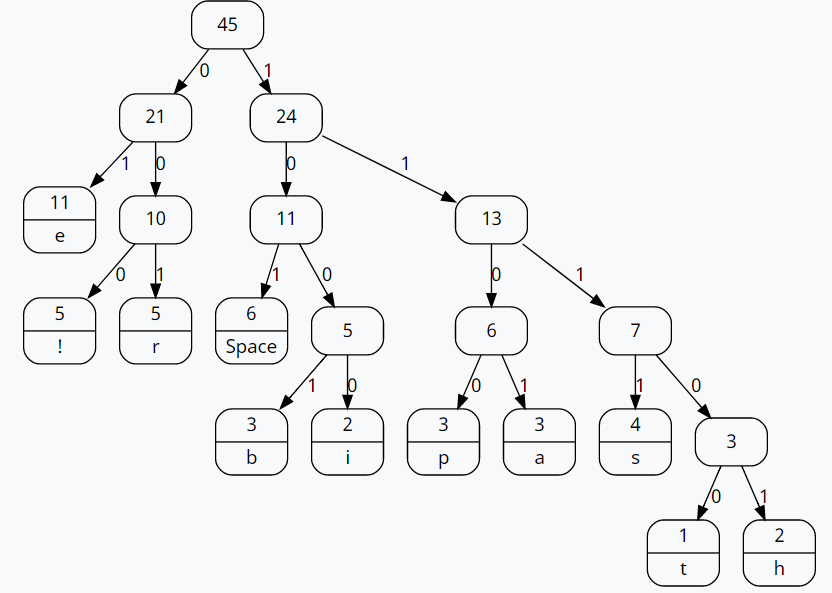
\includegraphics[scale=0.6]{hufftree}
\item There are:
\begin{lstlisting}
e = 01, ! = 000 ,r = 001 , _ = 101, b =1001, i = 1000, 
p = 1100, a = 1101, s = 1111, t = 11100, h = 11101
So compressed it uses 145 bits.
As a raw Ascii string it uses 352 bits.
\end{lstlisting}

\item 
\begin{lstlisting}
pete is here = 
1100 | 01 | 11100 | 01 | 101 | 1000 |
1111 | 101 | 11101 | 01 | 001 | 01

Compressed 39 bits
Raw ASCII 96 bits
\end{lstlisting}


\end{enumerate}

\clearpage

\section{(Q)Task 4 - Map and Reduce}
Solve the following using Javascript, for example in your browser’s developer console.\\
\begin{enumerate}
\item Map the list of numbers to a list of their square roots: [1, 9, 16, 100]
\item Map the list of words so each is wrapped in a <h1> tag: [“Intro”, “Requirements”, “Analysis”, “Implementation”, “Conclusion”, “Discussion”,
“References”]
\item Use map to uppercase the words (all letters): [“i’m”, “yelling”, “today”]
\item Use map to transform words into their lengths: [“I”, “have”, “looooooong”,
“words”]
\item Get the json file comics.json from the course site. Paste it into your
browser’s Javascript console. Use map to get all the image urls, and wrap
them in img-tags.
\item Use reduce to sum the array of numbers: [1,2,3,4,5]
\item Use reduce to sum the x-value of the objects in the array: [{x: 1},{x:
2},{x: 3}]
\item Use reduce to flatten an array of arrays: [[1,2],[3,4],[5,6]]
\item Use reduce to return an array of the positive numbers: [-3, -1, 2, 4, 5]
\item Optional: The accumulator function can obviously use objects outside of
itself. Use reduce to implement groupBy. For example:
p e o pl e = [
{name : ’ Rikke ’ , age : 4 6} ,
{name : ’ Michael ’ , age : 4 7} ,
{name : ’ Mathias ’ , age : 46}
] ;
should be turned into
g roupedPeople = groupBy ( pe ople , ’ age ’ ) ;
/*
g roupPe ople :
{
4 6: [
{name : ’ Rikke ’ , age : 4 6 } ,
{name : ’ Mathias ’ , age : 4 6 }
] ,
4 7: [
{name : ’ Michael ’ , age : 4 7 }
]
}
*/

\end{enumerate}

\section{(A)Task 4 - Map and Reduce}
\begin{enumerate}
\item 1
\begin{lstlisting}
>let arr = [1,9,16,100]
>let result = arr.map(Math.sqrt)
>result [1, 3, 4, 10]
\end{lstlisting}
\item 2
\begin{lstlisting}
>let arr = ["Intro","Requirements", "Analysis","Implementation",
"Conclusion","Discussion","References"]
>let h1 = arr.map(function(word){return "<h1>" + word + 
"<h1>"})
>h1 ["<h1>Intro<h1>", "<h1>Requirements<h1>",
 "<h1>Analysis<h1>", "<h1>Implementation<h1>",
 "<h1>Conclusion<h1>", "<h1>Discussion<h1>",
 "<h1>References<h1>"]
\end{lstlisting}
\item 3
\begin{lstlisting}
>let arr = ["i'm", "yelling", "today"]
>let up = arr.map(function(word){return word.toUpperCase()})
>up ["I'M", "YELLING", "TODAY"]
\end{lstlisting}
\item 4
\begin{lstlisting}
>let arr = ["I","have","looooooong","words"]
>let length = arr.map(function(word){return word.length})
>length [1, 4, 10, 5]
\end{lstlisting}
\item 5
\begin{lstlisting}
Couldn't find the file on the course page.
\end{lstlisting}
\item 6
\begin{lstlisting}
>let arr = [1,2,3,4,5]
>let sum = arr.reduce(function(summed,current){
return summed + current}
>sum 15
\end{lstlisting}
\item 7
\begin{lstlisting}
>let arr = [{x:1},{x:2},{x:3}]
>let sumobj = arr.reduce(function(summed,current){
return {x: summed.x + current.x}})
>sumobj {x: 6}
\end{lstlisting}
\clearpage
\item 8
\begin{lstlisting}
>let arr = [[1,2],[3,4],[5,6]]
>let flat = arr.reduce(function(a,b){return a.concat(b)})
>flat [1, 2, 3, 4, 5, 6]
\end{lstlisting}
\item 9
Er det meningen denne opgave skal løses med reduce og ikke filter? 
Er også usikker på om svaret skal være [1,2,3,4,5] eller [2,4,5]. 
Opgaven kan forstås på begge måder.
\begin{lstlisting}
>let arr =  [-3,-1,2,4,5]
>let posa = arr.filter(function(val){return val > 0})
posa [2, 4, 5]
\end{lstlisting}

\end{enumerate}


\end{document}
